\chapter{Coulomb explosion imaging}\label{ch:CEI}

\vspace{-1.5 em}
\begin{addmargin}[-0.5cm]{0cm}
  \minitoc
\end{addmargin}
\hrule
\vspace{1.5 em}

% The scope of this imaging method is to make measurements of the geometries of single molecules on a timescale faster than that of molecular motion ($10^{-15}$ seconds). Ultimately these images can be recorded in sequence to image the dynamics of a molecule. It works well for small molecules in the gas phase, a regime in which no other method has been viable.

% The method involves shooting a molecule in a vacuum chamber with two laser pulses, a pump pulse followed by a probe pulse after some time delay $\tau \ge 0$. The pump causes the molecule to undergo some change, then the more intense probe pulse strips off enough electrons from the molecule such that the molecule's individual atoms separate and repel each other ``explosively'' due to Coulomb repulsion. The further apart the atoms are repelled, the weaker the repulsion and eventually every atom reaches an asymptotic state of constant velocity. This all takes place in a constant electric field that accelerates all the atoms towards a time and position-sensitive detector. The detector can tell us how much time each atom took to reach it, and the position where the atom hit it. From this information, the atom’s (asymptotic) momentum can be calculated and then provided we know how to simulate the experiment in reverse, we can determine the initial geometry of the molecule just before it was hit by the pump pulse. By picking different values of $\tau$ and repeating the experiment many times for each $\tau$ we get a ``frame'' of the molecule's geometry at each $\tau$ , which may be placed in sequence to form a ``molecular movie'' of the change induced by the pump pulse.

% We are only interested in the molecular geometry, i.e. the relative positions of the atoms, not the absolute position of every atom. This reduces the dimensionality of our problem from $3n$ to $3n-6$ in both the geometry $\mathbf{g}$ and momentum vector $\mathbf{p}$. The geometry ``vector'' $\mathbf{g} \in \mathbb{R}^{3n-6}$ contains the molecule's bond lengths and bond angles, and the momentum ``vector'' $\mathbf{p} \in \mathbb{R}^{3n-6}$is a concatenation of momentum values in a specific convention. They both do not transform like vectors.

% While explosions proceed in a deterministic fashion, that is structures map bijectively to momentum measurements, the converse is not true. Two very different structures may produce the same momentum measurements. To make matters worse, there is no analytic solution to the problem and as the molecule grows, the problem of finding its structure becomes increasingly high dimensional. To combat this problem we will require the use of various mathematical and statistical methods. I first discuss some results from the theory of inverse problems to shed some general insight on these problems. I then follow with a discussion of optimization methods which may be used to tackle the problem for very small molecules. However, for full imaging of larger polyatomic molecules with an analysis of measurement error, Bayesian inference using Markov chain Monte Carlo methods is the way to go, which I discuss in the last chapter of this part.

% To find the initial geometry $\mathbf{g}_0$ that produced the measured asymptotic momentum $\mathbf{p}_\infty$, we make use of the fact that simulating the Coulomb explosion forward in time is easy. Let $\mathbf{p}(\mathbf{g}) : \mathbb{R}^{3n-6} \rightarrow \mathbb{R}^{3n-6}$ map an initial geometry $\mathbf{g}$ onto the asymptotic momentum vector $\mathbf{p}_\infty$ such a geometry produces upon Coulomb explosion. It simulates the explosion forwards in time by solving a set of $6n-12$ coupled first-order ODEs. Then casting this as an optimization problem, we seek the geometry $\mathbf{g}$ that minimizes the objective function $\left\| \mathbf{p}(\mathbf{g}) - \mathbf{p}_\infty \right\|_2^2$.

\section{What's the deal with Coulomb explosion imaging?}
Coulomb explosion imaging (CEI) is a general technique for studying the structure and ultrafast dynamics of small molecules in the gas phase, essentially by ionizing the molecule to induce fragmentation after which the positively-charged fragments repel each other in a \emph{Coulomb explosion}\footnotemark~ and the momentum vector of each fragment is measured. In principle, many claim that it is possible to retreive the molecular structure with just the momentum vectors, and we will a general method for doing this in the following chapters, however we will find out that this is a problem fraught with uncertainty to the point that geometry reconstructions cannot be trusted to provide us with insights into a molecule's structure. The momentum vectors may themselves be studied to infer molecular dynamics and changes in molecular structure.

\footnotetext{It is worth mentioning that the concept of a Coulomb explosion is indepdendent of CEI and refers to a cluster of many atoms repelling each other under their mutual Coulomb repulsion following ionization, for example by the intense electromagnetic field of a short laser pulse. Interestingly, a Coulomb explosion seems to be the mechanism responsible for the explosive reaction of alkali metals, such as sodium or potassium, with water, finally explaining the chemistry behind the classic high school experiment \citep{Mason15}.}

This does not sound like a technique of interest in the 21st century---the structure of virtually all small gas molecules is well known, what is left for CEI to tell us about? Producing molecular movies of ultrafast molecular dynamics is a main goal with imaging proton migration being a prototypical example. Once these ultrafast chemical processes are imaged and understood, it may be possible to control them. It can also tell us about non-classical molecular structures that elude other methods, such as that of \ch{C2H3+} and the Efimov state of the helium trimer (\ch{4He3}), and can serve more specialized purposes such as identifying the absolute geometry of molecular isomers.

Another reason for CEI's popularity may be that it promises direct and intuitive retreivals of molecular structure. Perhaps such physical reconstructions that can be understood by inspection satisfy our curiousity more so than complicated x-ray diffraction patterns. Certainly at least one author became interested with the prospect of \emph{seeing molecules} using lasers and explosions. CEI directly answers the question of ``what are we made of and what does it look like?'' first posed by the ancient Greeks and Indians, most famously by Democritus. The idea of the four classical elements: earth, air, fire, and water was proposed by many cultures to explain natural phenomena and the complexity of matter in terms of simpler entitites with some explanations being tied to atomism, the idea that matter was made of tiny, indivisible entities, such as Plato's association of the Platonic solids with the classical elements (see figure \ref{fig:platonicSolids}). While the ideas evolved over time, it was not until the 1600's that the theory was subject to experimental verification and eventually completely disproved. Even today, the classical elements are commonly employed and referred to in popular media. Such is the power of simple explanations.

\begin{figure}
  \centering
  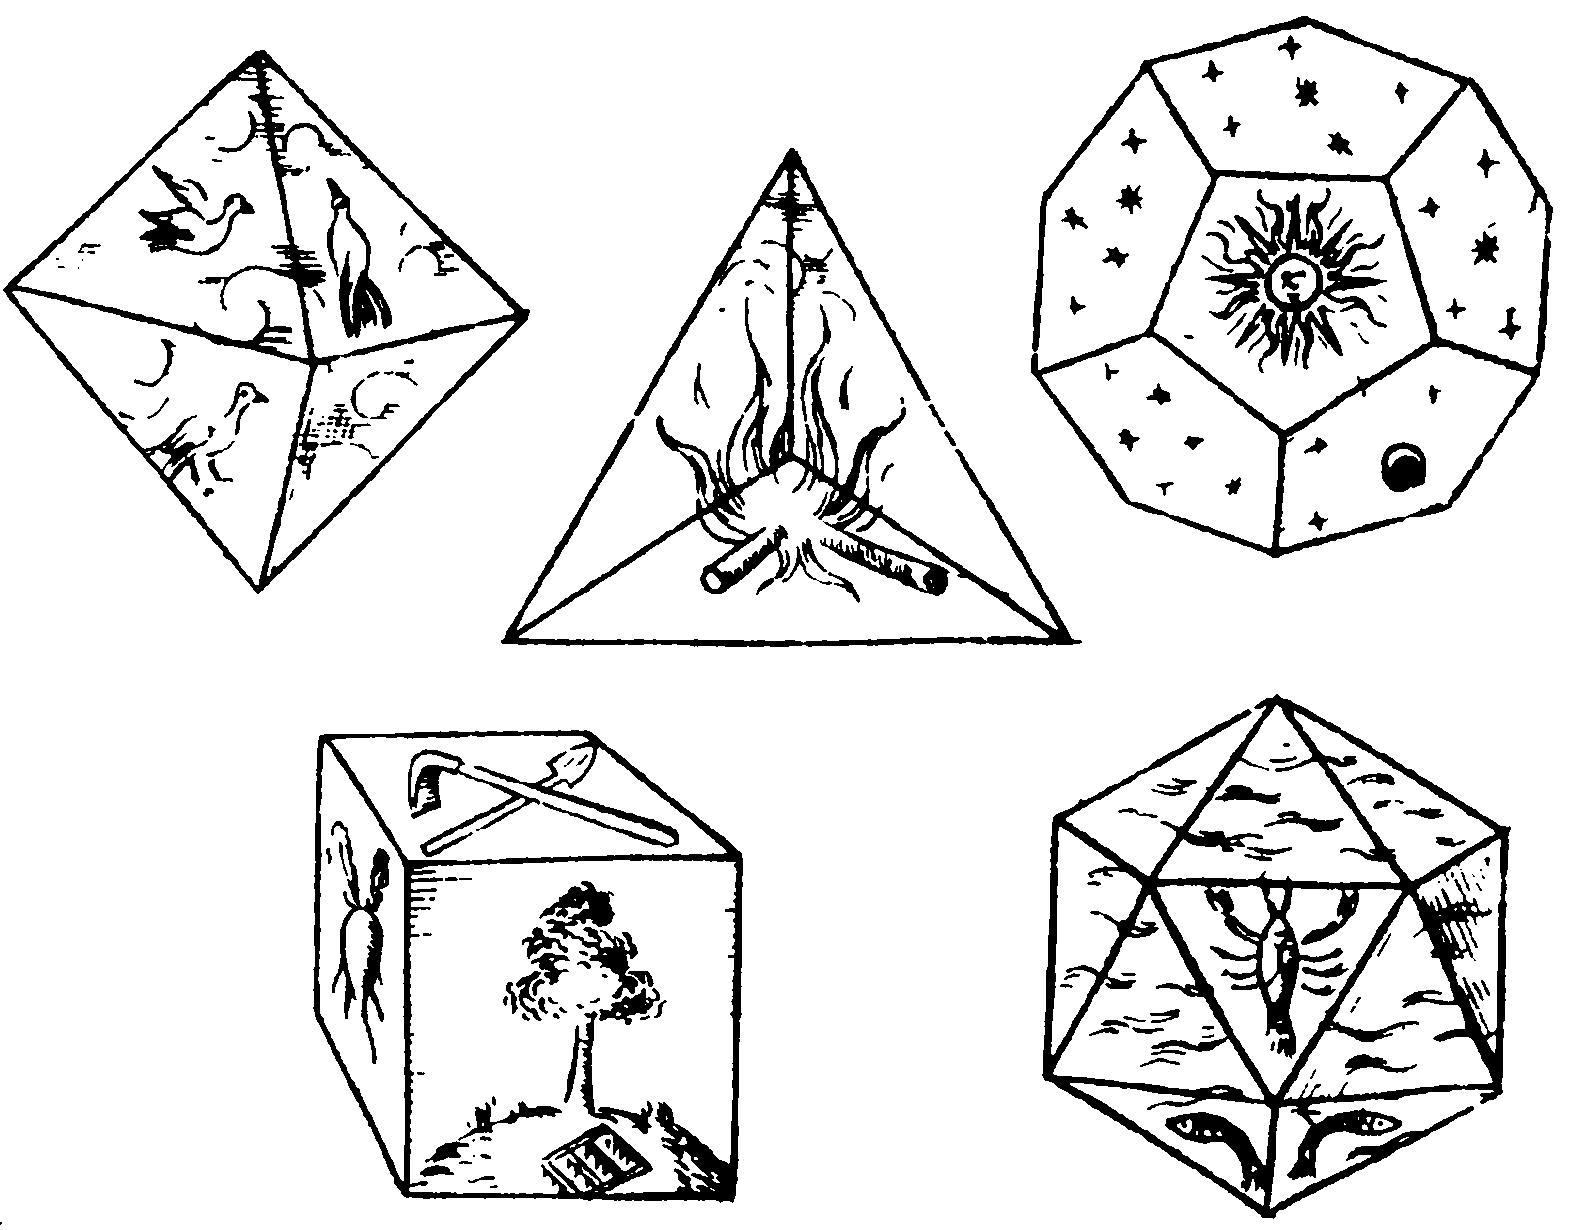
\includegraphics[width=\textwidth]{gfx/PlatonicSolids}
  \caption[The classical elements associated with the five Platonic solids.]
  {The classical elements associated with the five Platonic solids. Clockwise from the top left: the octahedron with air, tetrahedron with fire, dodecahedron with the universe, the isocehedron with water, and the cube with earth. Figure from \citet[Book 2, p. 53]{Kepler1619}. English translation available \citep{Kepler97}.}
  \label{fig:platonicSolids}
\end{figure}

\section{Physical principles and experimental outline} \label{sec:CEIphysics}
In pump-probe Coulomb explosion imaging (CEI) one ultrashort laser pulse is split into two pulses through the use an asymmetric beamsplitter. One of the pulses, the pump pulse, is usually much weaker than the other, the probe pulse. A time delay $\tau$ between the pulses is then created such that the pump pulse goes first and the probe pulse second. The job of the pump pulse will be to initiate some change in the molecule. One example could include an isomerization of the molecule. Thus the pump pulse ``pumps'' the molecule into some excited state. The job of the powerful probe pulse is to engulf the molecule in an intense enough laser field such that multiple electrons are stripped off of it. The molecule's individual atoms are left in a highly-charged state and begin to behave as individual point charges in a purely Coulombic potential. The entire process occurs in the presence of a constant electric field and so the positively-charged ions all accelerate upwards towards a time- and position-sensitive detector. Thus the probe pulse allows for the ``probing'' of the excited state.

\section{Molecular geometries seen using CEI}
The original CEI experiment is usually traced back to \citet{Vager89} in which the Coulomb explosion is initiated by passing a molecular beam through a thin foil. This may be because it was the first work suggesting that full molecular structures may be recovered by measuring the velocity (or momentum) vectors of the atomic fragments, and even reported on a non-classical molecular structure. However, previous works utilizing CEI do exist, even some significant works that report on molecular structures \citep{Kanter79}.

Ultrashort laser pulses\footnotemark as a means of inducing Coulomb explosions made their entrance in the 1980's where they were utilized to infer molecular dynamics using covariance mapping \citep{Frasinski89}. Highly charged ion impact is another method of inducing a Coulomb explosion, and was first done in the 1990's in parallel with the development of more sophisticated coincidence mapping techniques. Since then, the laser has emerged as the more popular tool and has further developed the coincidence mapping technique. There do exist other methods of inducing Coulomb explosions, for example, single photons from a synchrotron source utilizing the Auger effect, x-ray pulses from a free-electron laser source, or electron collision.

\footnotetext{In 1987, ultrashort would be referring to \SI{0.6}{\pico\s} laser pulses \citep{Frasinski87}.}

In this section we will trace the history of CEI back to the 1970's where it started with foil-induced fragmentation. We will then follow it's development to the present day where ultrashort laser pulses are the most popular means of performing CEI. Throughout we will focus solely on the achievements of CEI in determining molecular structures, and in creating molecular movies using these recovered structures.\footnotemark

\footnotetext{Much of the molecular dynamics are inferred in CEI from studying the distribution of the fragment momentum vectors (\eg~ through the use of Newton and Dalitz plots) and the distribution of kinetic energy carried away by each fragment. We will be focusing on the original aim of CEI, that is, to measure molecular structures.}

Interestingly, the first-ever mention of the term ``Coulomb explosion'' in the published literature comes from an unrelated study of the fine structure of singly ionized helium by \citet{Novick55}. They measured the energy difference of the $2 \, ^2 S_{1/2}$ and $2 \, ^2 P_{1/2}$ states of ionized helium as a sensitive test of quantum electrodynamics. Coulomb explosion (or space charge explosion) was the dominant ion removal mechanism which they accounted for in modeling the quenching rate\footnotemark of metastable $2 \, ^2 S_{1/2}$ ions by radio frequency radiation to describe the observed resonance lineshapes (spending two appendices on it).

\footnotetext{The term was more popular in decades past but simply means the extinction rate or loss rate of metastable ions.}

\subsection{Foil-induced dissociation}
CEI was first performed by passing a molecular beam containing the molecule of interest through a thin atomic film. Figure \ref{fig:foilExperiment} shows a schematic of such an experiment. While in the solid film, the probability for Coulomb scattering of the individual atomic nuclei is small due to their small size and consequently small interaction cross-section. However, the electrons will be scattered to very wide angles due to their interaction with the many electron clouds in the film. This process rapidly ionizes the molecule, typically within the first few atomic layers or the first femtosecond. The now highly ionized molecule exits the foil and rapidly dissociates into its consituent atomic fragments which repel eachother under their mutual Coulomb repulsion in what is termed a ``Coulomb explosion''.

\begin{figure}[H]
  \centering
  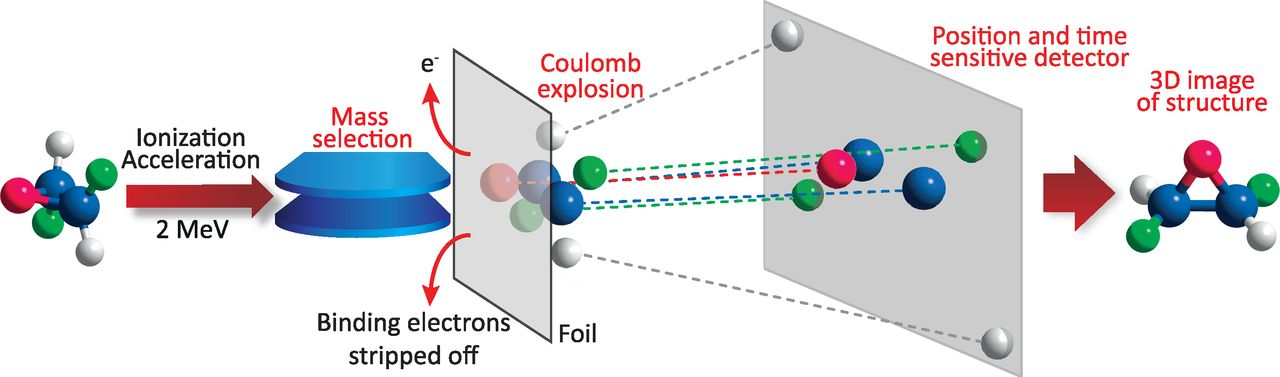
\includegraphics[width=\textwidth]{gfx/FoilExperiment}
  \caption[Schematic of a foil-induced Coulomb explosion imaging experiment.]
  {Schematic of a foil-induced Coulomb explosion imaging experiment. This specific experiment set out to measure the absolute configuration of atoms in a chiral molecule in the gas phase, which remains challenging. Early foil-induced CEI experiments can be described by this schematic except for the fact that they did not employ a mass selector and used a more primitive but still position-sensitive detector. The atomic fragment trajectories (dashed lines) assume that no rearrangement of the atoms occurs and that the system evolves under a Coulomb potential. From \citet{Herwig13}. Reprinted with permission from AAAS.}
  \label{fig:foilExperiment}
\end{figure}

The premise behind foil-induced CEI is that during this explosion, the atoms simply repel each other and do not rearrange, thus preserving the angles between them from the time they exit the foil to the time they are detected at a position and time-sensitive detector. As the potential energy of each pair of fragments $i,j$ is coverted to kinetic energy according to
\begin{equation}\label{eq:foilCEI}
\frac{4q_i q_j}{|\mathbf{r}_i - \mathbf{r}_j|} = \frac{\mu|\mathbf{V}_i - \mathbf{V}_j|^2}{2}
\end{equation}
it suggests that measurement of the asymptotic vector velocities completely defines the initial geometry of the molecule \citep{Vager89}. Here $q_i$, $\mathbf{r}_i$, and $\mathbf{V}_i$ are the charge, position vector, and velocity vector of the atomic fragment $i$ while $\mu$ is the reduced mass of the two-body system of fragments $i,j$.

\begin{figure}[H]
  \centering
  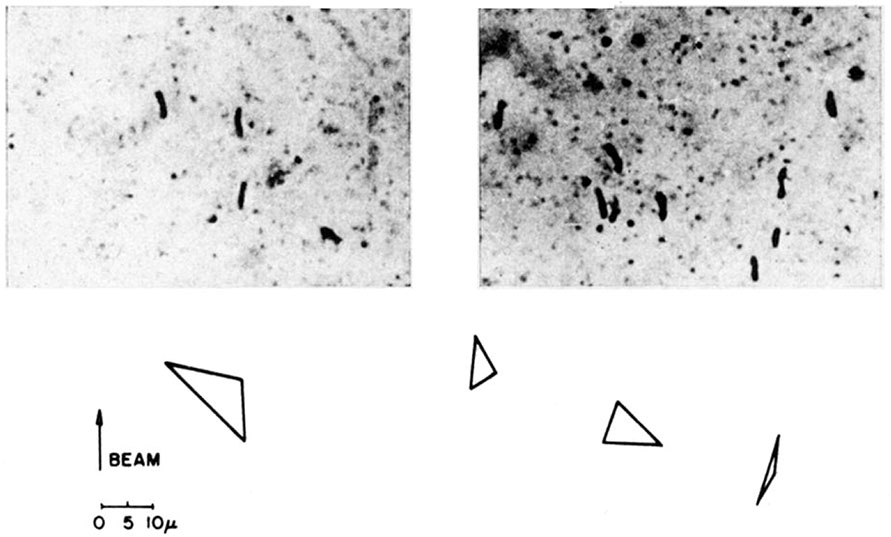
\includegraphics[width=\textwidth]{gfx/HydrogenTrimerReconstruction}
  \caption[Reconstructions of exploded \ch{H3+} following foil-induced dissociation.]
  {Reconstructions of exploded \ch{H3+} following foil-induced dissociation. On the top row are a couple of good photographs of exploded \ch{H3+} recorded on photographic emulsion at a tilt angle of $30\degree$. The bottom row shows a few reconstructions (normally projected) made by inspection from the photographs. The authors analyzed 350 such photographs and concluded that \ch{H3+} mainly exhibits an equalateral triangle geometry. From \citet{Gaillard78}. Reprinted with permission from APS.}
  \label{fig:hydrogenTrimer}
\end{figure}

The earliest example of a molecular geometry recovered using CEI is reported by \citet{Gaillard78}. They used the foil-induced Coulomb explosion to image the structure of the \ch{H3+} molecular ion, showing that it is mainly exhibits an equalaterial triangular shape in three completely different experiments.\footnotemark ~Figure \ref{fig:hydrogenTrimer} gives a few examples of the geometries they recovered.

\footnotetext{It is interesting to note that the experiment was repeated by three separate teams, then reported on coherently in one manuscript. Each team, having access to different equipment, produced separate pieces of data. It was the team in Rehovot, Israel that recorded the projections of the exploded ions while the others measured energy spectra and angular distributions.}

It is unclear how the idea for such an imaging experiment came to be, however it worth noting that \citet{Gaillard78} and co-authors have been studying the effects of molecular beams passing through thin foils for quite some time, mainly at Argonne National Laboratory. See for example their studies of wake potentials generated behind charged particles as they pass through a solid \citep{Gemmell75, Vager76PRL} and their study of the dissociation of fast \ch{HeH+} ions traversing thin foils \citep{Vager76PRA}. It seems quite reasonable that studying the dissociation of small molecules and the angular distribution of the fragments would inspire researchers to attempt to infer molecular structures using this data.

A better known CEI experiment was performed by \citet{Vager89} almost a decade later employing a $\sim$\SI{30}{\angstrom} carbon film. Their work was motivated by the opportunity of imaging non-classical molecular structures that more popular methods were incapble of seeing. They were also the first to suggest that measuring the velocity (or momentum) vectors of each fragment would be provide all the information required to describe the molecule's structure. Figure \ref{fig:C2H3geometry} shows one reconstruction based on the measured velocity vectors.

\begin{figure}
  \centering
  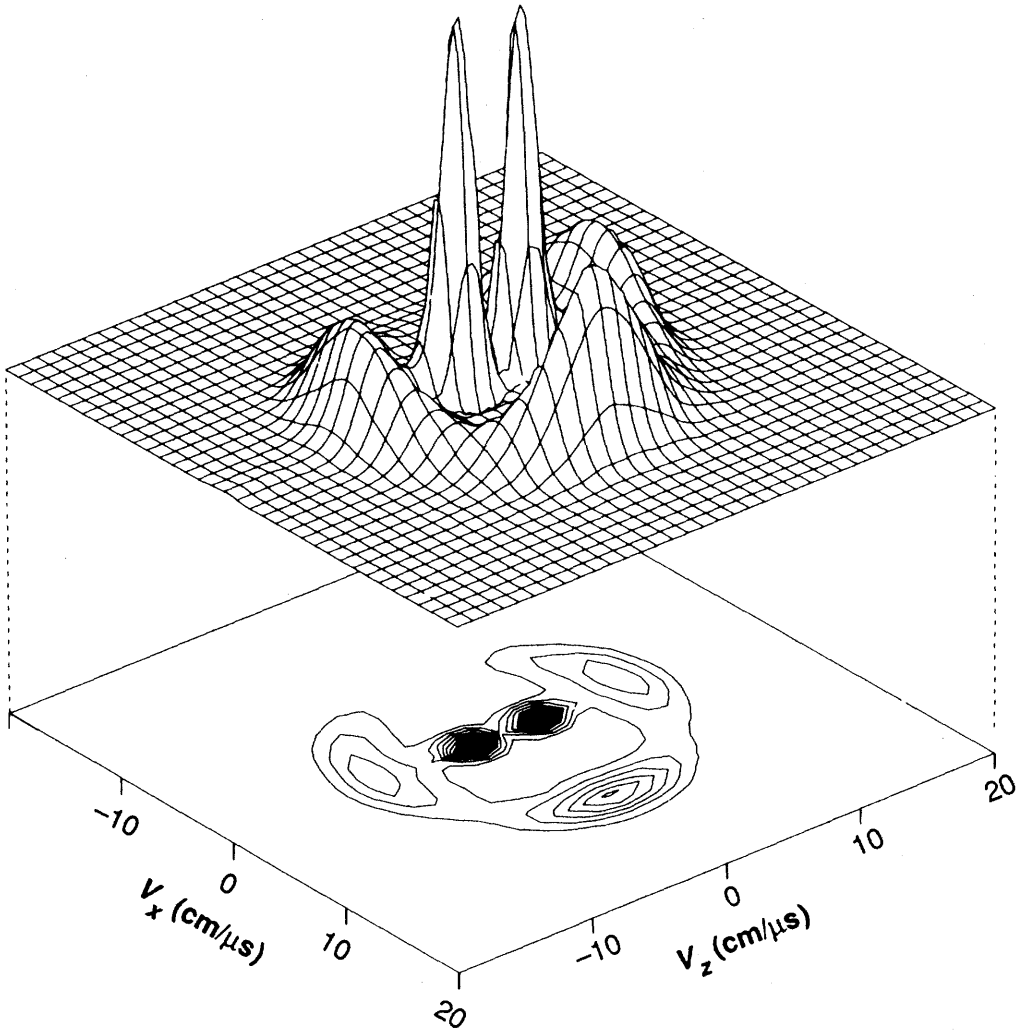
\includegraphics[width=\textwidth]{gfx/VagerPseudoGeometry}
  \caption[Reconstruction of \ch{C2H3+} following foil-induced dissociation.]
  {Reconstruction of \ch{C2H3+} following foil-induced dissociation. The densities of the fragment ions are plotted in a coordinate system defined by the final velocities of each particle (relative to the mean carbon-ion velocity). Assuming \eqref{eq:foilCEI} holds, this is an inference of the geometry, and quite a convincingly pretty one at that. The carbon ion densities were reduced by a factor of $5$ for display purposes. From \citet{Vager89}. Reprinted with permission from AAAS.}
  \label{fig:C2H3geometry}
\end{figure}

However, they do not perform any geometry reconstruction and report their fragment ion densities in a coordinate system defined by the asymptotic velocity of each particle, and claim that it is a direct measurement of the square of the multidimensional wave function of a many-body system.

The promise of recovering molecular geometries in this simple fashion seems quite empty after glancing at the published literature in the past few decades. While foil-induced CEI has found some uses and produced some interesting work in recent years\footnotemark~, for the purposes of studying molecular structures and dynamics, the ultrafast laser shortly thereafter became the tool of choice for CEI as we will discuss in section \ref{sec:laserCEI}. The reason for the scarcity of foil-induced CEI experiments in the published literature is mainly due to its limitations.

\footnotetext{This includes imaging the rovibrational wave functions of \ch{H2-} and \ch{D2-} by studying the kinetic energy relased by the fragments \citep{Jordon-Thaden11, Herwig13PRA}, and imaging the absolute configuration of chiral molecules in the gas phase by studying the measured velocity vectors of the fragments with Newton plots \citep{Herwig13}.}

Of course, there are some assumptions that must hold for a complete and accurate recovery of the initial geometry, which we shall discuss in section \ref{sec:CEIphysics}. However, just by inspection of the schematic in figure \ref{fig:foilExperiment} we can see that no rearrangement of the atoms must occur\footnotemark~ and that the molecular system must evolve on the Coulomb potential, which requires the rapid stripping of many electrons off the atom. Thus CEI becomes increasingly difficult to perform with larger molecules so it is best used to study smaller molecules. However, it is precisely these small molecules in the gas phase that need to be studied using CEI as they cannot be probed using other more established methods. Moreover, many smaller molecules may exhibit non-Coulombic behaviour unless placed into a highly charged state, which may be impossible depending on the apparatus in use. For foil-induced CEI in particular, a molecular beam must be prepared, and this may prohibit the study of many molecules that cannot be prepared as such.

\footnotetext{While this is the case for many smaller molecules, it is not true for some of the popular targets. For example, a triatomic molecule may dissociate into a single atom and a diatomic rotor, which rotates before dissociating into two atoms.}

\subsection{Imaging with ultrashort laser pulses}\label{sec:laserCEI}

\subsubsection*{Attempt at an analytical solution}
\index{Classical imaging formula}
\index{Coulomb explosion imaging!Classical imaging formula}
Before taking a tour of the molecular geometries recovered using laser-induced CEI, it is worth mentioning that \citet{Nagaya04} have attempted to arrive at an analytical solution for calculating molecular geometries from measured momentum vectors. They were able to derive a \emph{classical imaging formulae} giving the image of the squared vibrational wavefunction inverted from the momentum distribution of the atomic ions for the Coulomb explosion of a diatomic molecule, a linear symmetric triatomic molecule, and a linear asymmetric triatomic molecule. They are able to derive similar formulae for the diatomic and linear, symmetric, triatomic molecule, but the more general case of the asymmetric, linear, triatomic molecule proves much more formidable.\footnotemark~ The bulk of their article focuses on that case, deriving a three-dimensional classical imaging formula in terms of Jacobi and hyperspherical coordinates then reducing it to two dimensions. An extension to three dimensions for bent triatomic molecules is promised but could not be found in the published literature.

As an example, their formula for the Coulomb explosion of a diatomic molecule $AB$
\begin{equation}
|\Psi_\mathrm{image}(R_I)|^2 = S(p) \frac{1}{P_\mathrm{ion}(R_I)} \sqrt{\frac{\mu q_A q_B}{8\pi\epsilon_0 R_I^3}}
\end{equation}
where $S(p)$ is the momentum distribution measured in the asymptotic region (when the atomic fragments are far apart and barely interact), $P_\mathrm{ion}(R_I) = |T_\mathrm{ion}(R_I)|^2$ is the ionizatin probability, $mu$ is the reduced mass of the diatomic molecule, $q_A$ and $q_B$ are the electric charges on atoms $A$ and $B$ respectively, and $R_I = \mu q_A q_B/2\pi\epsilon_0 p^2$ seems to be turning point of the Frank-Condon factor.

They proceed to compare their ``classical'' reconstructions for the vibrational wavefunction of a helium trimer system to the predictions of the quantum theory, noting small discrepencies. It seems that similar formulae were derived and actually used in previous studies \citep{Bandrauk01,Chelkowski02}.

\footnotetext{While a highly commendable effort, their unsaid conclusion seems to be that this is an intractable problem as their research group seems to have gone silent on this problem and the very few citations to this work are in the context of the difficulty of the problem.}

\subsubsection*{Inferring dynamics from energy spectra and momentum vector distribtuions}
Due to the difficulty of recovering the molecular geometries, the structures and dynamics of small molecules are usually inferred from the kinetic energy spectra of the fragments and their momentum vector distributions (usually studied using Newton and Dalitz plots).

\subsubsection*{Experimental reconstructions}
\citet{Legare05structure,Legare05dynamics} were the first to use ultrashort laser pulses (\SI{8}{\fs}) and CEI to report on molecular structures and dynamics. Figure \ref{fig:SO2-232structure} shows a reconstruction of \ch{SO2} using the \ch{SO2^{7+}} charge state. To obtain the structures, they assume the explosion system evolves under a purely Coulombic potential and use optimization methods to make guesses at the structure that most accurately reproduces the observed data consistent with minimizing a least-squares objective function. Treating the geometry reconstruction as an optimization problem is exactly what we do in chapter \ref{ch:optimization}. However, dissapointly, they trivialize the solution to a couple of sentences and fail to report the optimization methods employed, sidestepping the nuances of the reconstruction process that we will discuss in chapters \ref{ch:lookupTable}--\ref{ch:bayesian}. The nuances include the existence, in some cases, of multiple molecular structures producing the same momentum vector distribution (dubbed degenerate geometries) and the high sensitivity of the reconstructed initial geometry to uncertainties in the momentum vectors leading to very uncertain geometries in some cases. Without knowledge of the optimization methods used, it is impossible to tell whether appropriate methods were used. We will show that this is an ill-posed inverse problem, or rather, a constrained nonlinear optimization problem calling for optimization methods that are typically outside the scope of introductory optimization textbooks.

\begin{figure}
  \centering
  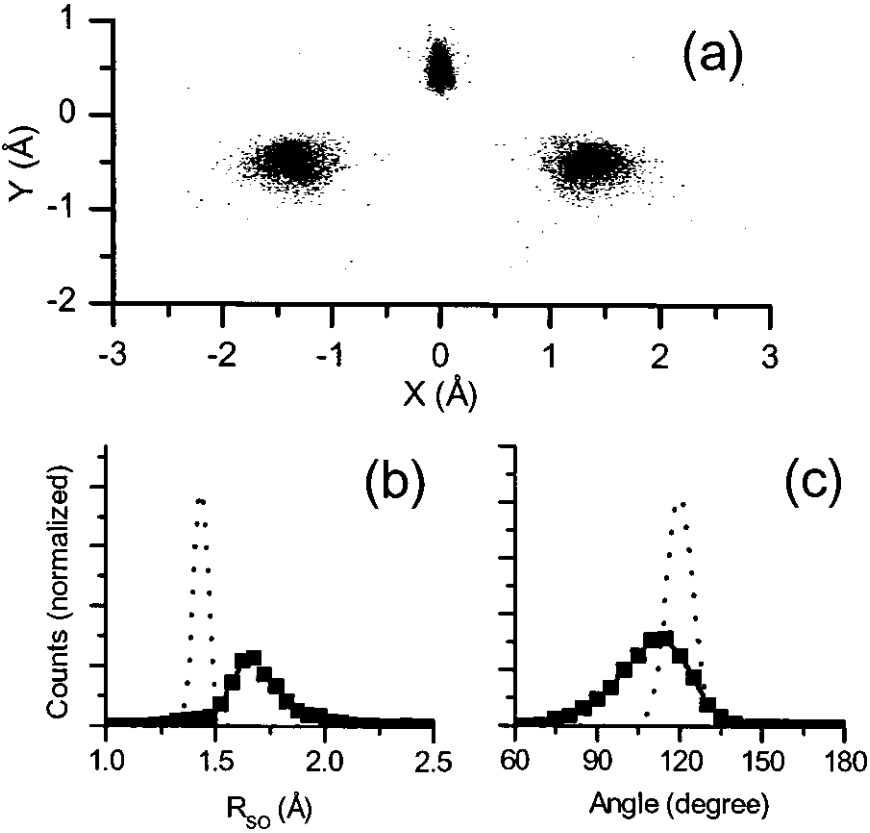
\includegraphics[width=\textwidth]{gfx/LegareSO2-232Structure}
  \caption
  [Molecular structure of \ch{SO2} using the \ch{SO2^7+} charge state.]
  {(a) Molecular structure of \ch{SO2} using the \ch{SO2^7+} charge state (\ch{SO2^7+ $\rightarrow$ O^2+ + S^3+ + O^2+}). The center of mass is at $x=0$, $y=0$, and the $y$-axis is the bisector of the angle. While an intuitive way to plot geometries, we will show that such a plot can hide unphysical correlations in the reconstructed geometries. (b) Radial distribution and (c) angular distribution of the reconstructed geometries with the dotted lines showing the expected distributions for the $\nu=0$ stationary state structure of \ch{SO2}. While the results again make intuitive sense, it would be interesting to see whether the radial distributions of both bond lengths to help ascertain the robustness of their reconstruction method. These marginal distributions are typically of the greatest interest but we will show that they can be used to hide unphysical correlations, and that joint distributions should be reported. From \citet{Legare05structure}. Reprinted with permission from APS.}
  \label{fig:SO2-232structure}
\end{figure}

They also claim to have imaged vibrating \ch{D2^+} and dissociating \ch{SO2^2+} and \ch{SO2^3+} however they provide no more than a couple of dissociation frames and infer the transient \ch{D2^+} bond length from kinetic energy release ratios as a function of pump-probe time delay \citep{Legare05dynamics}.

\citet{Gagnon08} reported the reconstruction of dichloromethane (\ch{CH2Cl2}) using a home-made \footnotemark stochastic-based simulated annealing algorithm that globally optimizes the molecular spatial configuration. They discuss uncertainties but are only able to obtain the structure in five cases.

\footnotetext{There is nothing wrong with writing your own code here but nonconvex optimization algorithms are tricky to get right and professional optimization libraries (both proprietary and open-source) do exist. At least the methods and source code are publicly available \citep{Gagnon06}.}

\begin{SCfigure}
  \centering
  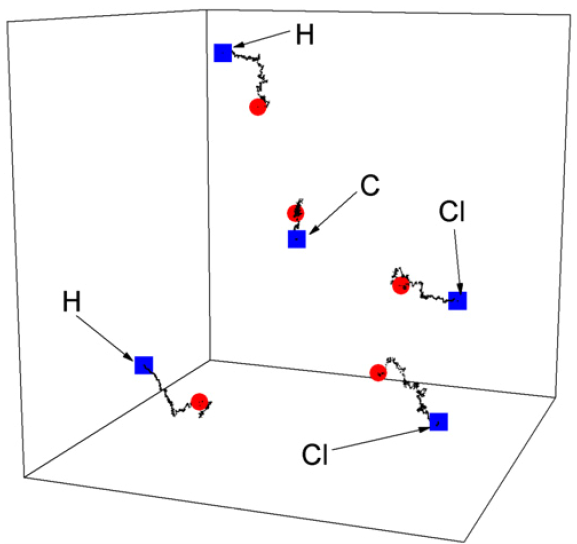
\includegraphics[width=0.5\textwidth]{gfx/CH2Cl2Geometry}
  \caption
  [Geometry of \ch{CH2Cl2}.]
  {Geometry of \ch{CH2Cl2}. From \citet{Gagnon08}. Reprinted with permission from IOP.}
  \label{fig:CH2Cl2geometry}
\end{SCfigure}

\index{Lookup table}
The most impressive and trustworthy geometry reconstruction effort so far is perhaps the imaging of the Efimov state of the helium trimer by \citet{Kunitski15}, coming full circle to the very first images of the hydrogen trimer \citep{Gaillard78}.

\begin{figure}
  \centering
  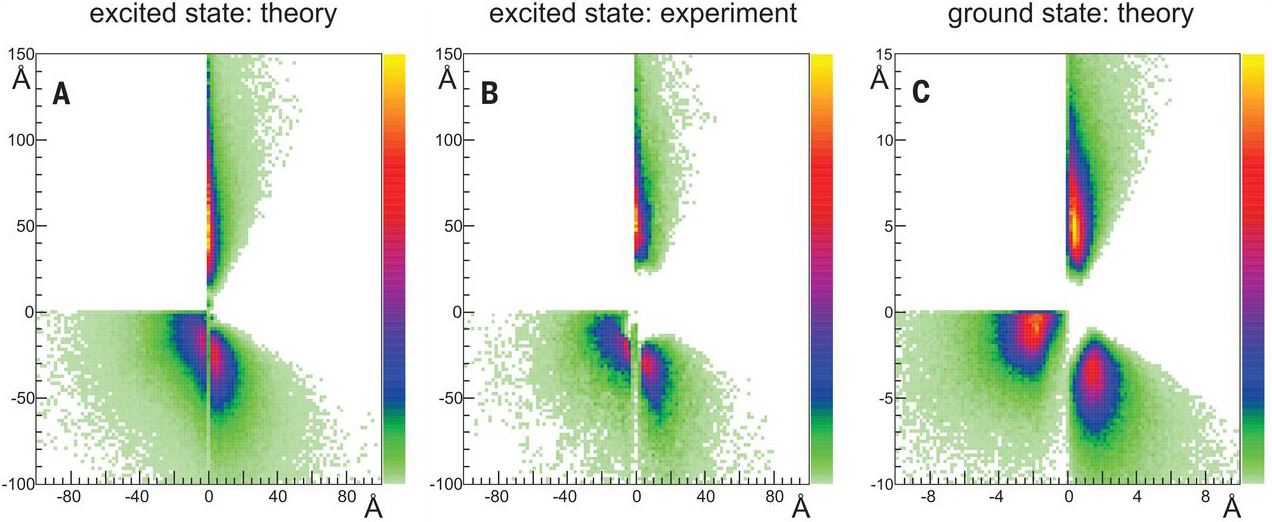
\includegraphics[width=\textwidth]{gfx/HeliumTrimerReconstruction}
  \caption[Helium trimer reconstruction.]
  {Helium trimer reconstruction.}
  \label{fig:heliumTrimerReconstruction}
\end{figure}

\subsection{Other methods and uses}

\subsection{Molecular movies}
Molecular movies are of course not only of interest in physics and chemistry as a means of probing fundamental processes, but also in the biological sciences where molecular structure play a crucial role in determining the function of biomolecules such as proteins. However, the molecules of interest there are much too large to be studied by any of the previous techniques. Thus molecular movies in the biological sciences tend to be annotated computer simulations amalgamated from multiple studies. That said, they are very impressive pieces of work.

A particularly impressive movie by \citet{Cheung12} showcases the process of RNA polymerase transcription and goes on for over six minutes.